% !TEX encoding = UTF-8
% !TEX TS-program = pdflatex
% !TEX root = ../Tesi.tex
% !TEX spellcheck = it-IT

%************************************************
\chapter{Diagramma E-R}
\label{cap:diagramma}
%************************************************

Una volta analizzate le specifiche del progetto per il quale si vuole realizzare il database, si identificano e si descrivono le singole entità e le loro associazioni.

\section{Descrizione delle entità}
	
	\subsection{Utente}
	
		\begin{figure}[h]
			\centering
			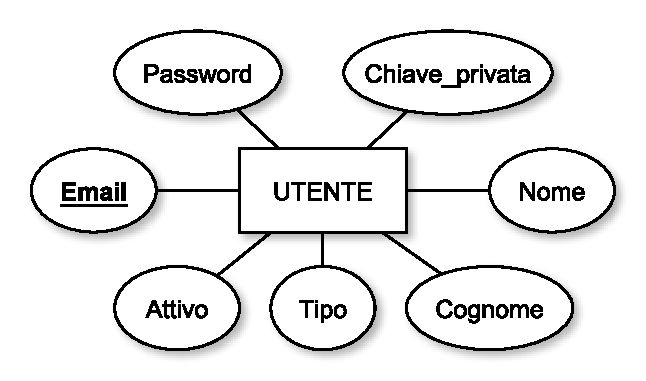
\includegraphics[width=0.5\textwidth]
			{immagini/01-utente}
			
			\caption{Entità Utente}
		\end{figure}
		
		Entità che rappresenta un generico utente dell'applicazione. L'utente si distingue in \emph{Registrato} e \emph{Amministratore}.
		
		\subsubsection*{Descrizione Attributi}
		
		\begin{description}
			
			\item[Email]
			Chiave primaria dell'entità che identifica univocamente l'utente.
			
			\item[Password]
			Stringa alfanumerica con lunghezza di 32 caratteri. Il valore di tale attributo viene generato cifrando, mediante la funzione crittografica MD5, la password inserita dall'utente.
			
			\item[Chiave privata]
			Stringa alfanumerica con lunghezza di 32 caratteri. Il valore di tale attributo viene generato cifrando, mediante la funzione crittografica MD5, il Timestamp di registrazione dell'utente.
			
			\item[Nome]
			Il valore di tale attributo viene inserito dall'utente.
			
			\item[Cognome]
			Il valore di tale attributo viene inserito dall'utente.
			
			\item[Tipo]
			Carattere singolo. Serve per identificare il tipo di utente registrato nel database. Tale attributo può assumere i seguenti valori:
			A~(Amministratore), G~(Gestore~squadra), R~(Arbitro).
			
			\item[Attivo]
			Booleano. Serve per determinare se un utente è attivo oppure no, permettendo a quest'ultimo di accedere al sito.
			
		\end{description}
	
	\subsection{Amministratore}
	
		\begin{figure}[h]
			\centering
			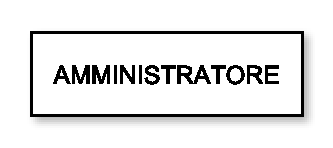
\includegraphics[width=0.3\textwidth]
			{immagini/02-amministratore}
			
			\caption{Entità Amministratore}
		\end{figure}
		
		Specializzazione dell'entità utente, eredita tutti gli attributi dell'entità utente. Serve per rappresentare gli utenti aventi i privilegi di ``ROOT''.
	
	\subsection{Registrato}
	
		\begin{figure}[h]
			\centering
			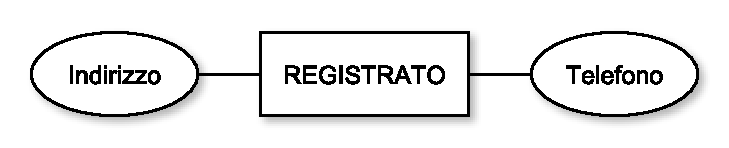
\includegraphics[width=0.6\textwidth]
			{immagini/03-registrato}
			
			\caption{Entità Registrato}
		\end{figure}
		
		Specializzazione dell'entità utente, eredita tutti gli attributi dell'entità utente. Serve per rappresentare gli utenti Gestori Squadra e Arbitri che possono accedere all'applicazione Web. Tale entità può essere creata solo dall'amministratore.
		
		\subsubsection*{Descrizione Attributi}
		
		\begin{description}
			
			\item[Indirizzo]
			
			
			\item[Telefono]
			
			
		\end{description}
	
	\subsection{Arbitro}
		
		\begin{figure}[h]
			\centering
			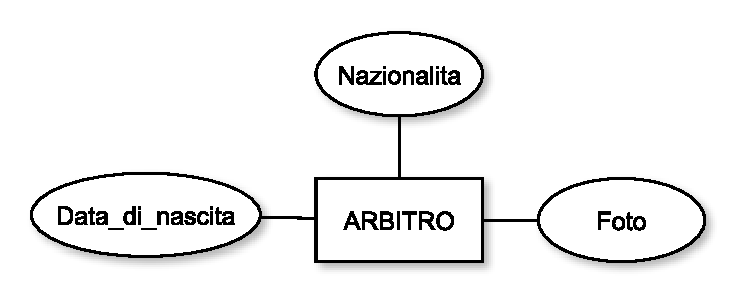
\includegraphics[width=0.6\textwidth]
			{immagini/04-arbitro}
			
			\caption{Entità Arbitro}
		\end{figure}
		
		Specializzazione dell'entità Registrato, eredita tutti gli attributi dell'entità utente. Serve per rappresentare il tipo di utente Arbitro. Tale entità può essere creata solo dall'amministratore.
		
		\subsubsection*{Descrizione Attributi}
		
		\begin{description}
			
			\item[Data di nascita]
			Indica la data di nascita dell'arbitro.
			
			\item[Nazionalita]
			
			
			\item[Foto]
			
			
		\end{description}
	
	\subsection{Gestore Squadra}
	
		\begin{figure}[h]
			\centering
			
\includegraphics[width=0.3\textwidth]
			{immagini/05-gestore-squadra}
			
			\caption{Entità Gestore Squadra}
		\end{figure}
		
		Specializzazione dell'entità Registrato, eredita tutti gli attributi dell'entità Registrato e Utente. Serve per rappresentare il tipo di utente Gestore Squadra. Tale entità può essere creata solo dall'amministratore.
	
	\subsection{Torneo}
	
		\begin{figure}[h]
			\centering
			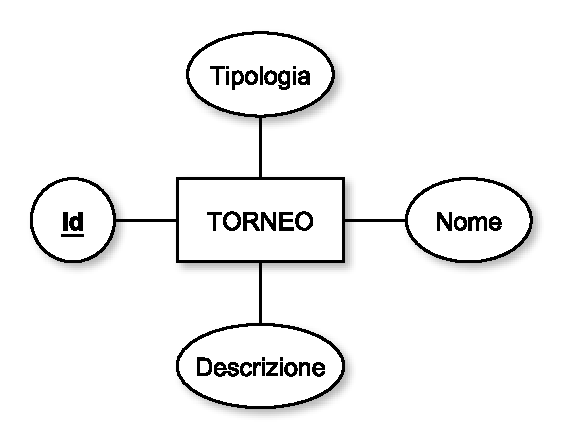
\includegraphics[width=0.5\textwidth]
			{immagini/06-torneo}
			
			\caption{Entità Torneo}
		\end{figure}
		
		Entità che rappresenta un torneo in svolgimento o già svolto. Può essere di due tipi: ad eliminazione diretta o all'italiana.
		
		\subsubsection*{Descrizione Attributi}
		
		\begin{description}
			
			\item[Id]
			Intero. Chiave primaria dell'entità che identifica univocamente il torneo.
			
			\item[Tipo]
			Serve per distinguere i due tipi di torneo.
			
			\item[Nome]
			
			
			\item[Descrizione]
			Informazioni aggiuntive relative al torneo (storia, luogo, sponsor, ecc.).
			
		\end{description}
	
	\subsection{Partita}
		
		\begin{figure}[h]
			\centering
			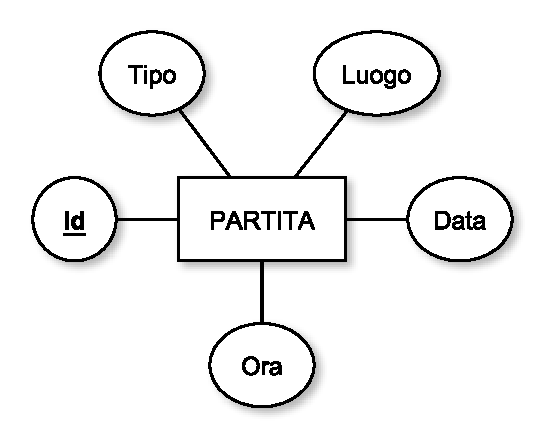
\includegraphics[width=0.5\textwidth]
			{immagini/07-partita}
			
			\caption{Entità Partita}
		\end{figure}
		
		\subsubsection*{Descrizione Attributi}
		
		\begin{description}
			
			\item[Id]
			Intero. Chiave primaria dell'entità che identifica univocamente una partita.
			
			\item[Tipo torneo]
			Identifica da che tipo di torneo derivano le partite. Serve per gestire in due modi diversi le classifiche.
			
			\item[Luogo]
			
			
			\item[Data]
			
			
			\item[Ora]
			
			
		\end{description}
	
	\subsection{Referto}
		
		\begin{figure}[h]
			\centering
			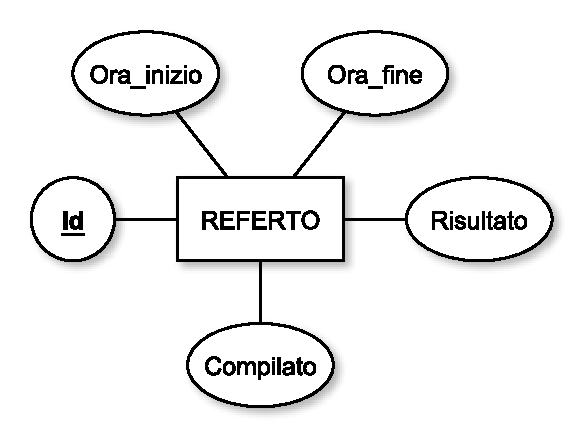
\includegraphics[width=0.5\textwidth]
			{immagini/08-referto}
			
			\caption{Entità Referto}
		\end{figure}
		
		Entità che rappresenta il referto di una determinata gara.
		
		\subsubsection*{Descrizione Attributi}
		
		\begin{description}
			
			\item[Id]
			Intero. Chiave primaria dell'entità che identifica univocamente un referto.
			
			\item[Ora inizio]
			Orario effettivo di inizio della partita.
			
			\item[Ora fine]
			Orario effettivo di fine della partita.
			
			\item[Risultato]
			Risultato finale dell'incontro
			
			\item[Compilato]
			Serve per capire se il referto è stato compilato o meno.
			
		\end{description}
	
	\subsection{Squadra}
	
		\begin{figure}[h]
			\centering
			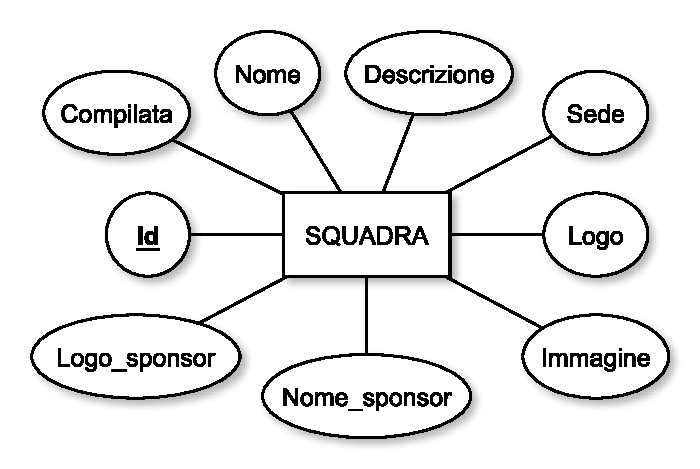
\includegraphics[width=0.6\textwidth]
			{immagini/09-squadra}
			
			\caption{Entità Squadra}
		\end{figure}
		
		Entità che rappresenta una squadra all'interno dell'applicazione Web.
		
		\subsubsection*{Descrizione Attributi}
		
		\begin{description}
			
			\item[Id]
			Intero. Chiave primaria dell'entità che identifica univocamente la squadra.
			
			\item[Compilata]
			Serve per identificare se un gestore squadra ha compilato la squadra. Se la squadra non è stata compilata, la prima volta che si accede all'applicazione web si dovranno fornire i dati richiesti. Se non si forniscono i dati della squadra non si può svolgere nessuna attività.
			
			\item[Nome]
			Nome legale della società.
			
			\item[Descrizione]
			Informazioni aggiuntive relative alla squadra.
			
			\item[Sede]
			Sede legale della società.
			
			\item[Logo]
			Identifica il logo/simbolo della squadra.
			
			\item[Immagine]
			Identifica la foto della squadra.
			
			\item[Nome sponsor]
			Identifica il nome dello sponsor ufficiale della squadra.
			
			\item[Logo sponsor]
			Identifica il logo dello sponsor ufficiale della squadra.
			
		\end{description}
	
	\subsection{Classifica}
	
		\begin{figure}[h]
			\centering
			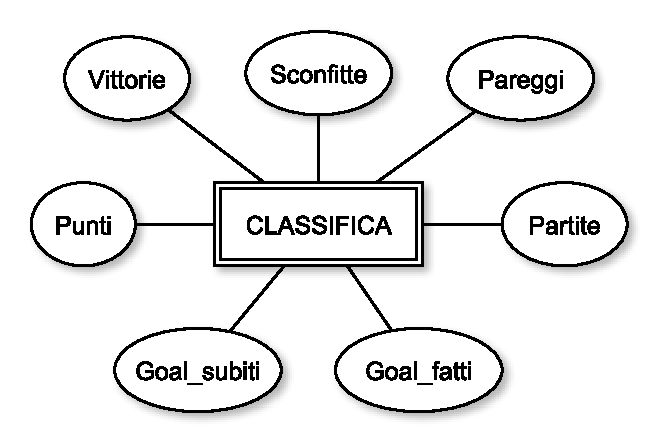
\includegraphics[width=0.6\textwidth]
			{immagini/10-classifica}
			
			\caption{Entità Classifica}
		\end{figure}
		
		Entità debole in quanto non ha propri attributi chiave, rappresenta la classifica di un determinato torneo.
		
		\subsubsection*{Descrizione Attributi}
		
		\begin{description}
			
			\item[Punti]
			Punti totalizzati fino a quel momento da una determinata squadra in un determinato torneo.
			
			\item[Vittorie]
			Numero totale delle partite giocate da una squadra in un determinato torneo.
			
			\item[Sconfitte]
			Dati per il monitoraggio delle partite disputate da una squadra fino a quel momento.
			
			\item[Pareggi]
			Dati per il monitoraggio delle partite disputate da una squadra fino a quel momento.
			
			\item[Partite]
			Dati per il monitoraggio delle partite disputate da una squadra fino a quel momento.
			
			\item[Goal fatti]
			Rappresenta il totale dei goal fatti dai giocatori di una determinata squadra in un torneo.
			
			\item[Goal subiti]
			Rappresenta il totale dei goal subiti da una squadra nelle partite di un torneo.
			
		\end{description}
		
	\subsection{Giocatore}
	
		\begin{figure}[h]
			\centering
			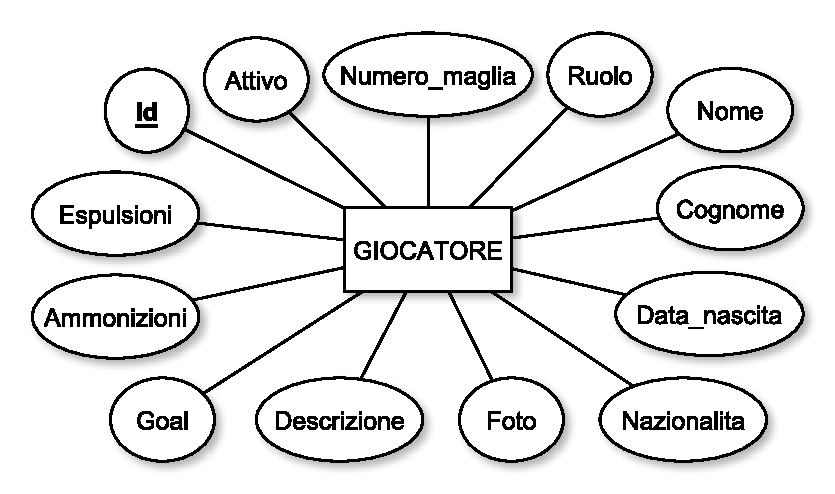
\includegraphics[width=0.8\textwidth]
			{immagini/11-giocatore}
			
			\caption{Entità Giocatore}
		\end{figure}
		
		Entità debole che rappresenta un determinato atleta/giocatore.
		
		\subsubsection*{Descrizione Attributi}
		
		\begin{description}
			
			\item[Id]
			Chiave parziale che identifica univocamente i vari giocatori di una squadra.
			
			\item[Attivo]
			Determina se un giocatore è attivo oppure no.
			
			\item[Numero maglia]
			Numero maglia con cui il giocatore prende parte alle partite.
			
			\item[Ruolo]
			Ruolo che il giocatore interpreta in campo.
			
			\item[Nome]
			
			
			\item[Cognome]
			
			
			\item[Data di nascita]
			
			
			\item[Nazionalita]
			
			
			\item[Foto]
			Immagine che raffigura il giocatore.
			
			\item[Descrizione]
			Informazioni aggiuntive relative al giocatore.
			
			\item[Goal]
			Dati per monitorate il rendimento di ogni singolo giocatore.
			
			\item[Ammonizioni]
			Dati per monitorate il rendimento di ogni singolo giocatore.
			
			\item[Espulsioni]
			Dati per monitorate il rendimento di ogni singolo giocatore.
			
		\end{description}

\section{Descrizione delle associazioni}
	
	\subsection{Ha}
	Associazione presente tra Torneo e Classifica.
	
	\subsection{Presente}
	Associazione presente tra Squadra e Classifica.
	
	\subsection{Composta}
	Associazione presente tra Squadra e Giocatore.
	
	\subsection{Gestisce}
	Associazione presente tra Gestore Squadra e Squadra.
	
	\subsection{Riferito}
	Associazione presente tra Partita e Referto.
	
	\subsection{Gestisce Registrato}
	Associazione presente tra Registrato e Amministratore.
	
	\subsection{Gestisce Torneo}
	Associazione presente tra Amministratore e Torneo.
	
	\subsection{Partecipa}
	Associazione presente tra Torneo e Squadra.
	
	\subsection{Cartellino}
	Associazione presente tra Arbitro e Giocatore.
	
	\subsection{Marcatore}
	Associazione presente tra Referto e Giocatore.
	
	\subsection{Scelto}
	Associazione ternaria presente tra Arbitro, Amministratore e Partita.
	
	\subsection{Formazione}
	Associazione ternaria presente tra Squadra, Giocatore e Referto.
	
	\subsection{Giocano}
	Associazione ternaria presente tra Partita, Torneo e Squadra.
	

\section{Il modello E-R completo}
Per il modello E-R completo si veda la figura \vref{fig-modello-ER}.


\begin{figure}[h]
	\centering
	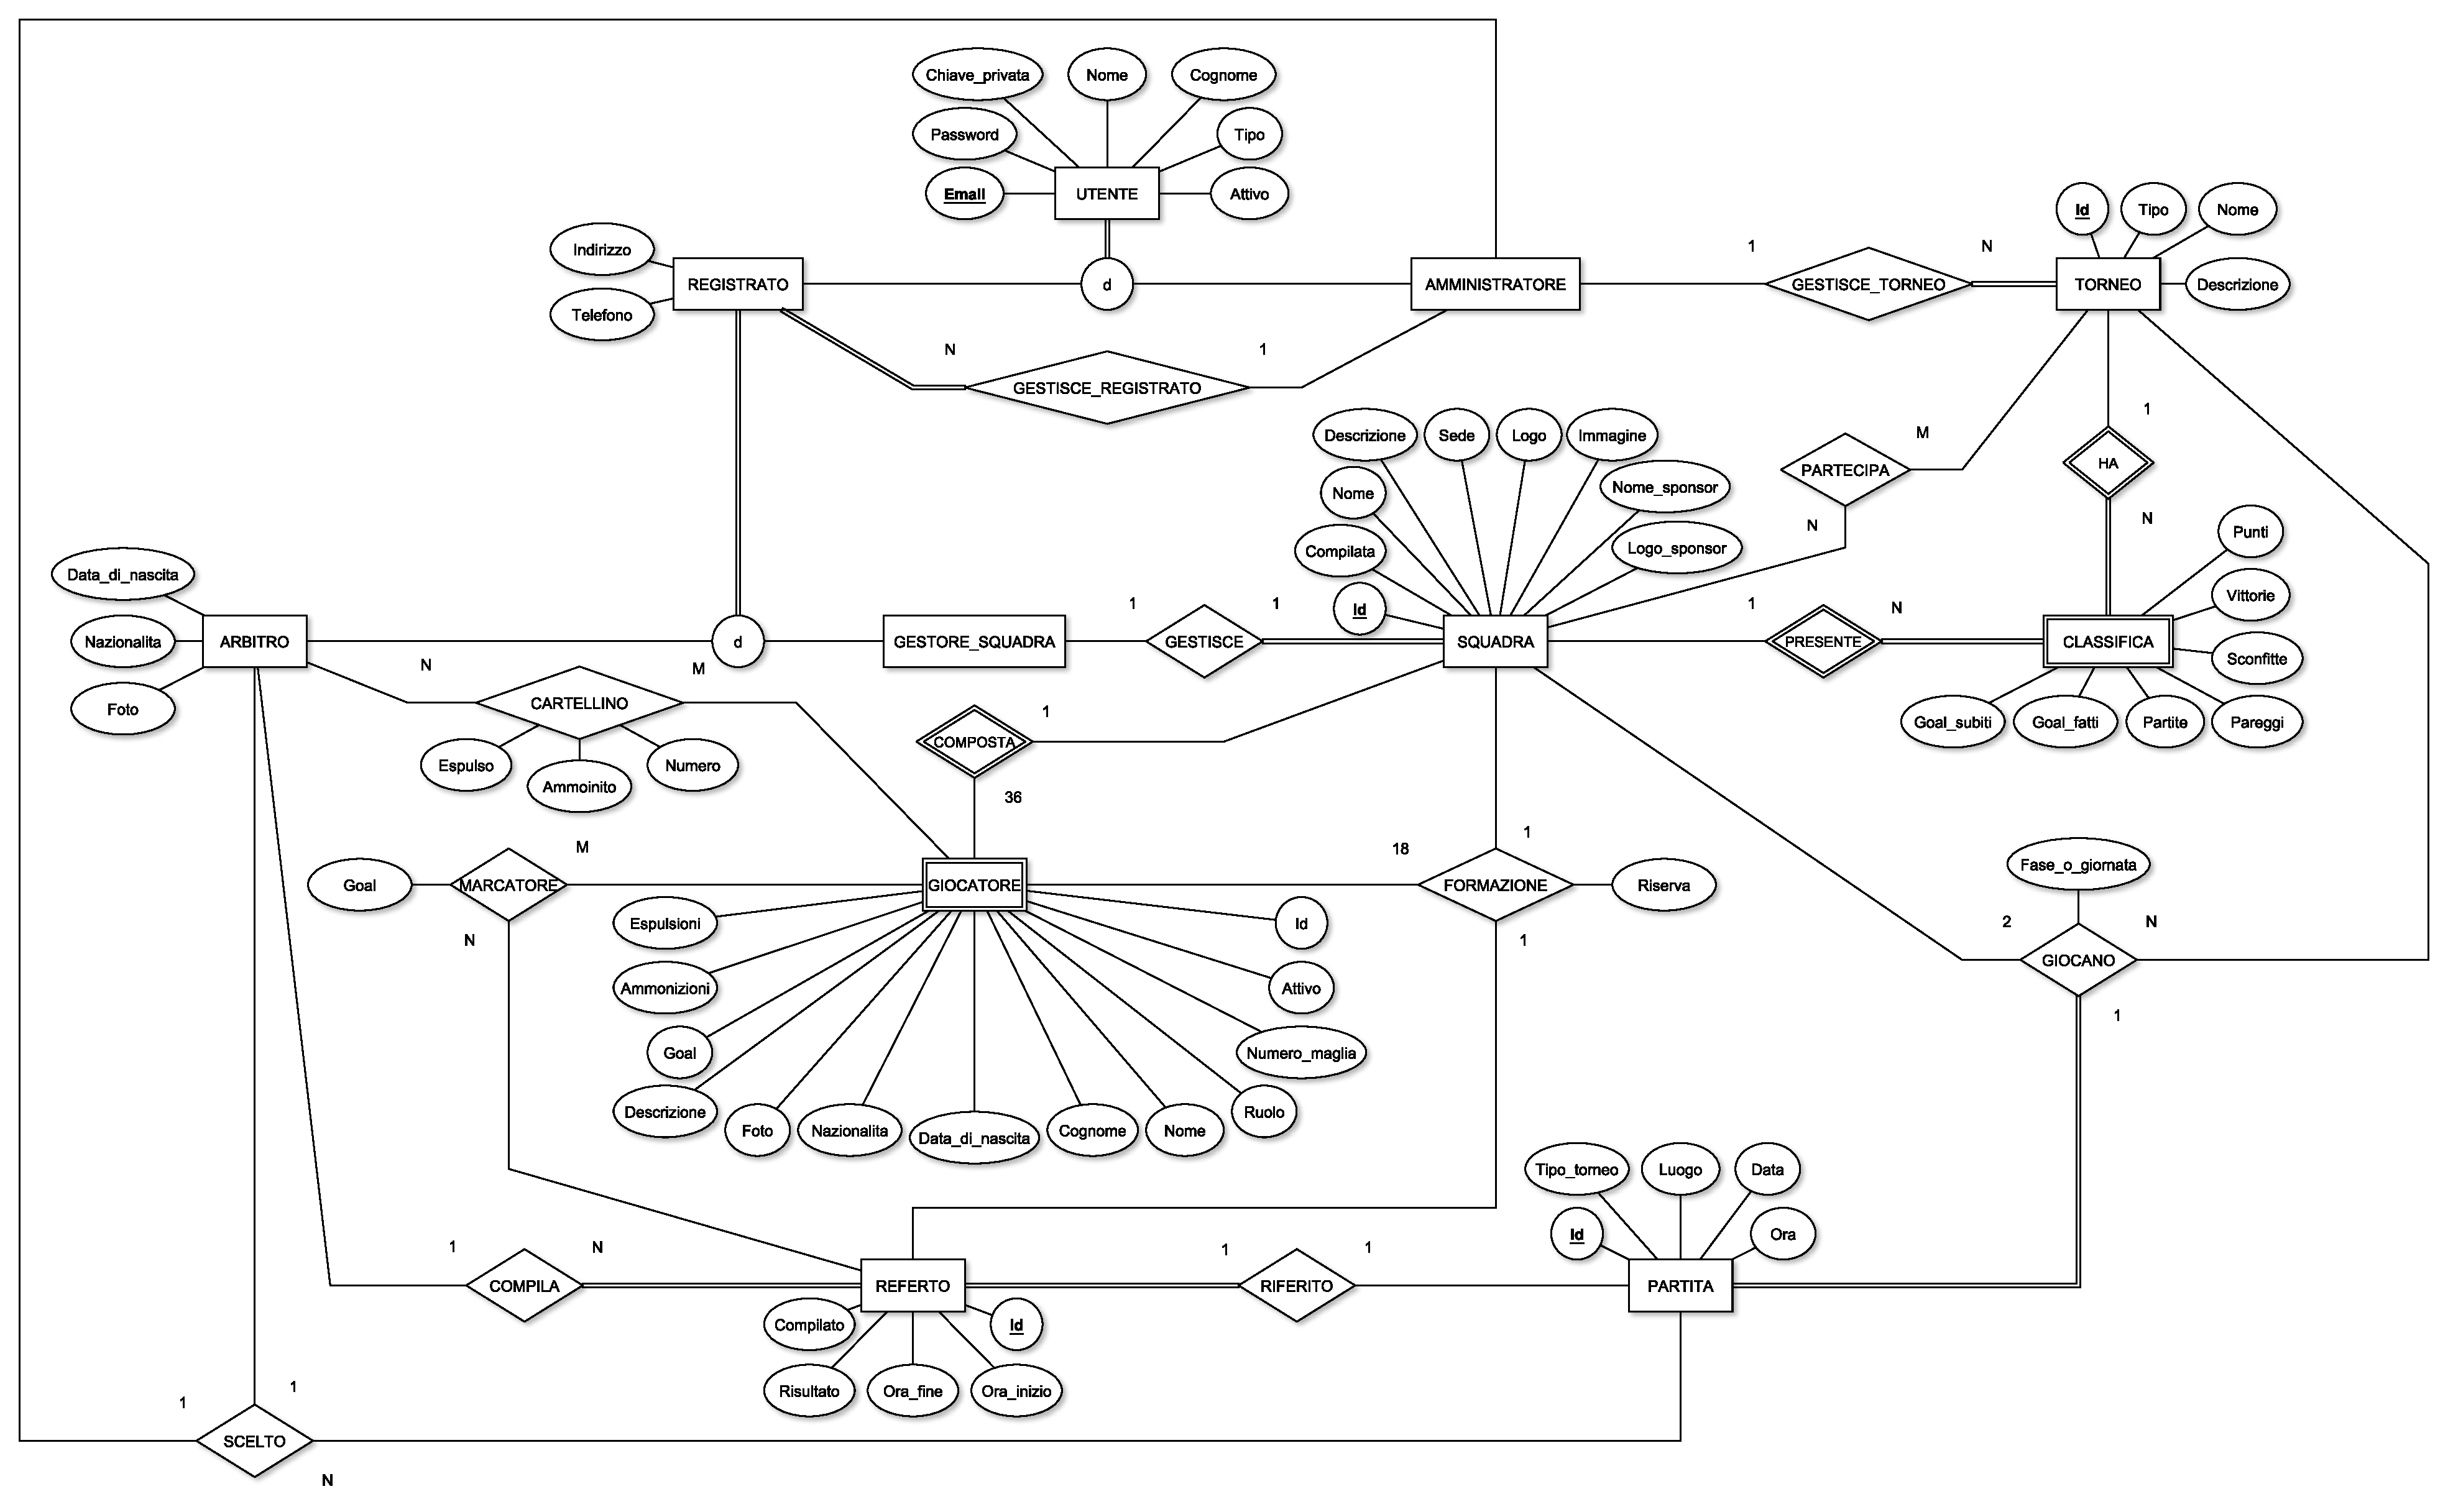
\includegraphics[height=1\textwidth,
	angle=90]
	{immagini/diagramma-ER-completo}
	
	\caption{Schema E-R completo}
	
	\label{fig-modello-ER}
\end{figure}	